\section{Visualizando del resultado}
\label{sec:visualizing-results}

La visualización del resultado es esencial para comprender el resultado de la detección del
deadlock. Por esta razón invertimos tiempo en investigar diferentes formas de lograr el mismo
resultado, con y sin una instalación local necesaria para que fuera lo más fácil de usar posible.

Estas instrucciones también se pueden encontrar en el
\texttt{README}\footnote{\url{https://github.com/hlisdero/cargo-check-deadlock/blob/main/README.md}}
del repositorio.

\subsection{Localmente}

Para ver la representación \acrshort{MIR} del código fuente, se puede compilar el código con la
flag correspondiente: \Rustinline{rustc --emit=mir <path_to_source_code>}

Es importante tener en cuenta que la cadena de herramientas nocturna puede producir \acrshort{MIR}
diferentes en comparación con la versión estable del compilador. Remitimos al lector a la
Sec. \ref{sec:rust-nightly} para más información.

Para graficar una red en formato \Rustinline{.dot}, instale la herramienta dot siguiendo las instrucciones
de la página web de GraphViz\footnote{\url{https://graphviz.org/download/}}.

Ejecute \Rustinline{dot -Tpng net.dot -o outfile.png}
para generar una imagen PNG a partir del archivo de salida \Rustinline{.dot}.

Ejecute \Rustinline{dot -Tsvg net.dot -o outfile.svg} para generar una imagen SVG a
partir del archivo de salida \Rustinline{.dot}.

Encontrará más información y otros posibles formatos de
imagen en la documentación\footnote{\url{https://graphviz.org/doc/info/command.html}}.

\subsection{En línea}

Para ver la representación \acrshort{MIR} del código fuente,
se puede utilizar el Rust Playground\footnote{\url{https://play.rust-lang.org/}}.

Debe seleccionar la opción ``MIR'' en lugar de ``Run'' en el menú desplegable.
Tenga en cuenta que debe utilizarse la versión nightly en lugar de la versión estable de \emph{rustc}.

Para graficar un resultado DOT dado,
la herramienta Graphviz Online\footnote{\url{https://dreampuf.github.io/GraphvizOnline/}}
ofrece una alternativa fiable a las herramientas instaladas localmente.
Existen alternativas como Edotor\footnote{\url{https://edotor.net/}}
o SketchViz\footnote{\url{https://sketchviz.com/new}}.

\subsection{Depuración (\textit{Debugging})}
\label{sec:debugging}

El programa soporta los flags de verbosidad definidas en el crate
\texttt{clap\_verbosity\_flag}\footnote{\url{https://docs.rs/clap-verbosity-flag/latest/clap\_verbosity\_flag/}}.
A modo de ejemplo, ejecutar el programa con la bandera \texttt{-vvv} imprime mensajes de \emph{debug} que
pueden ser útiles para localizar qué línea de la \acrshort{MIR} no se está traduciendo correctamente.

Entonces deberá invocar la herramienta del siguiente modo:

\Rustinline{cargo check-deadlock <path_to_program>/rust_program.rs -vvv}

El comprobador de modelos \acrshort{LoLA} admite la impresión de una ``witness path''
que muestra una secuencia de disparos de transición que conducen a un deadlock.
Esto es extremadamente útil cuando se extiende la funcionalidad del traductor y
el análisis de la red de Petri no coincide con el resultado esperado para un programa dado.

En el repositorio se incluye un práctico script llamado \texttt{run\_lola\_and\_print\_witness\_path.sh}
para imprimir la ruta testigo de un archivo \texttt{.lola}.
La Fig. \ref{fig:lola-output} ilustra el resultado
de ejecutar el script en el archivo mostrado en el Listado \ref{lst:double-lock-deadlock-mir}.

\begin{figure}[!htb]
  \centering
  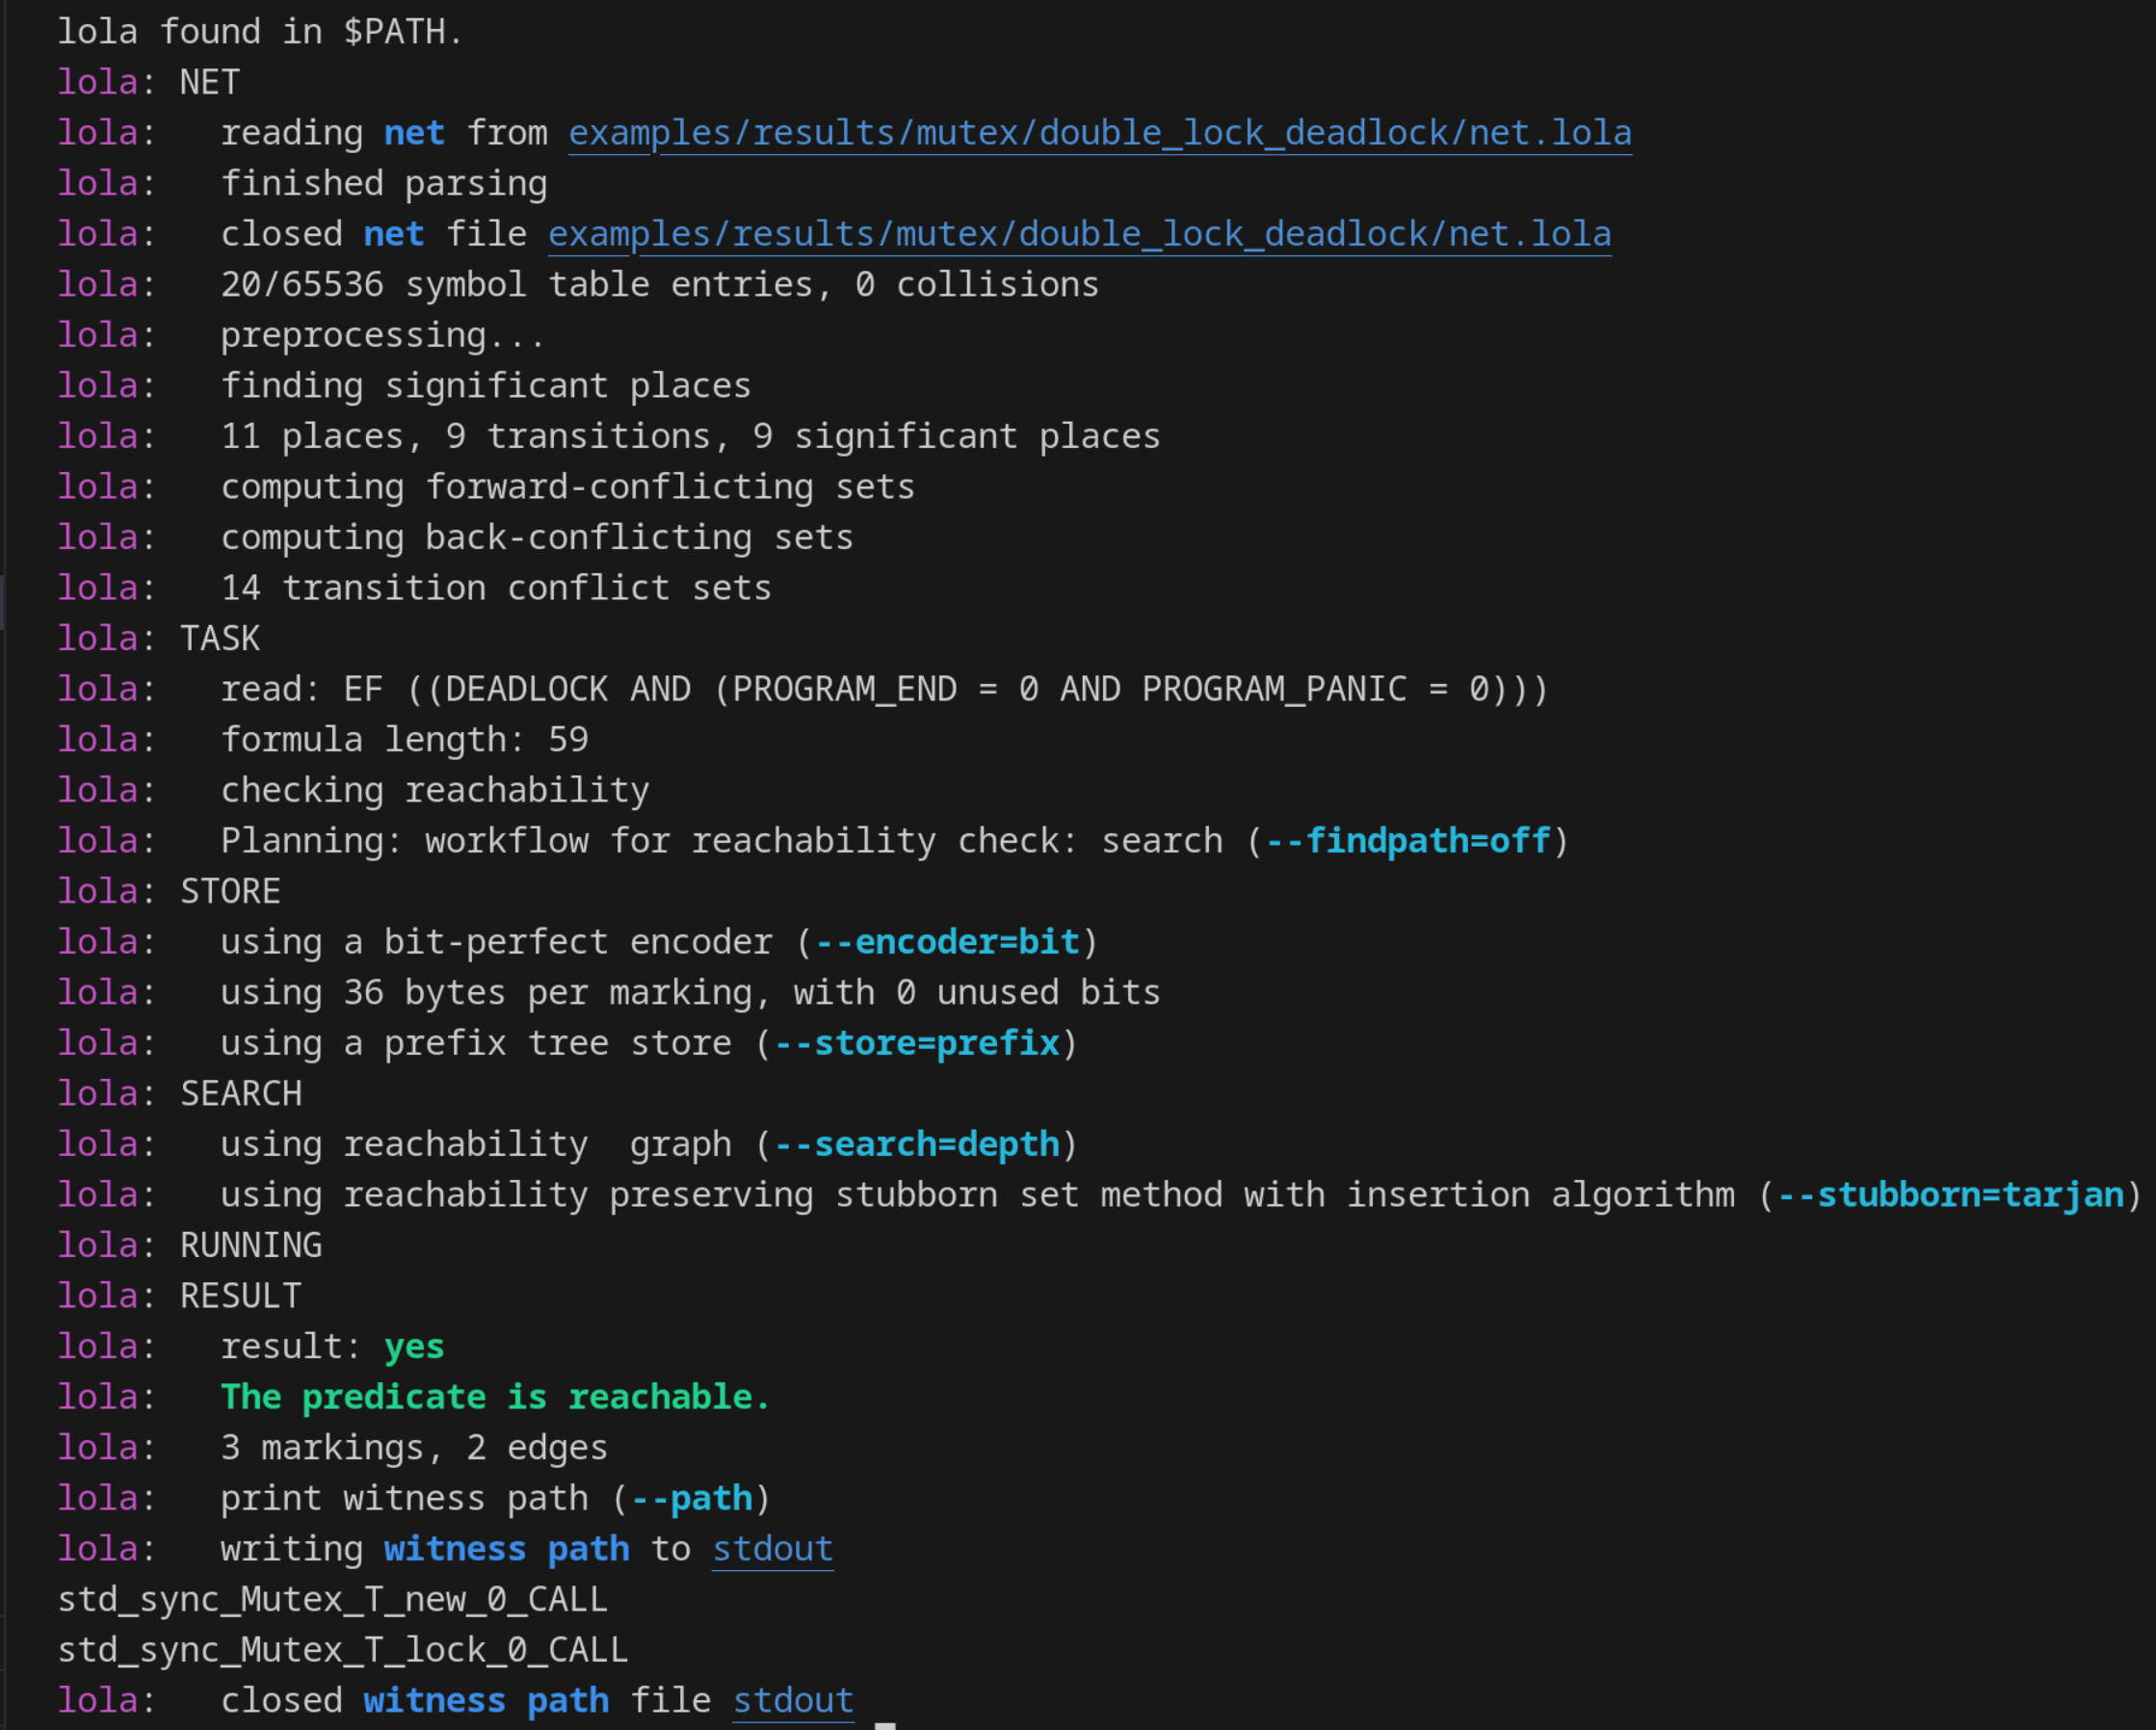
\includegraphics[width=\linewidth]{lola-output.png}
  \caption{Salida de la ruta testigo generada por LoLA para el programa del Listado \ref{lst:double-lock-deadlock}.}
  \label{fig:lola-output}
\end{figure}